\documentclass[12pt]{article}
\usepackage{graphicx}
\usepackage{amssymb}
\usepackage{epstopdf}
\usepackage{amsmath}
\usepackage{multicol}
\usepackage{tcolorbox}
\usepackage{geometry}
\usepackage{enumitem}
\usepackage{fancyhdr}

\DeclareGraphicsRule{.tif}{png}{.png}{`convert #1 `dirname #1`/`basename #1 .tif`.png}

\textwidth = 6.5 in
\textheight = 9 in
\oddsidemargin = 0.0 in
\evensidemargin = 0.0 in
\topmargin = -23pt
\headheight = 0.0 in
\headsep = 0.0 in
\parskip = 0.2in
\parindent = 0.0in
\pagestyle{fancy}
\pagenumbering{gobble}

\newtheorem{theorem}{Theorem}
\newtheorem{corollary}[theorem]{Corollary}
\newtheorem{definition}{Definition}
%\includegraphics [height=50mm, width=50mm]{PathInt.jpg}
\title{Title} 

\begin{document}
%INSTRUCTOR NOTES
%No warm-up on quiz days. If wanted, today's warm-up would be solving equations.
 Name:
 \begin{center}\large{2.5 Concavity}\end{center}

Warm-up: Imagine this bottle filling with water all the way to the top. Sketch a possible graph of the height of the water in the bottle as a function of the volume of water in the bottle.

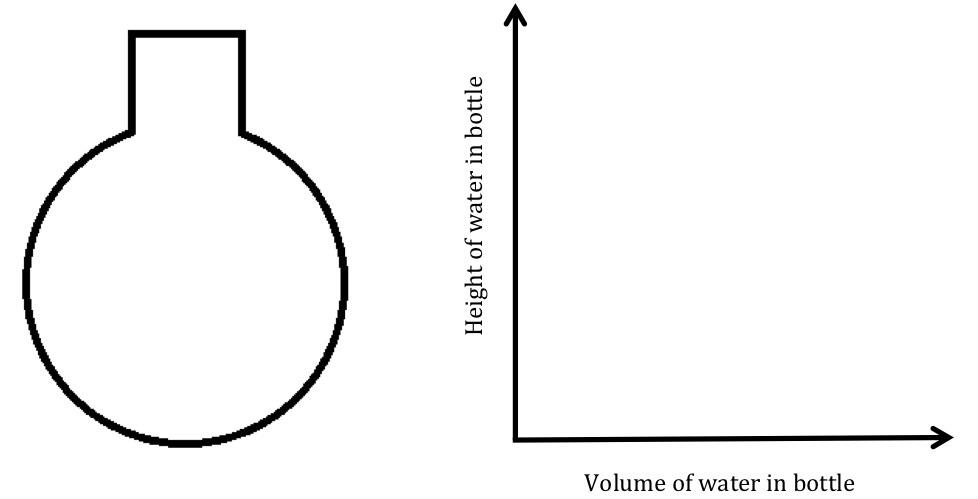
\includegraphics [height=80mm, width=160mm]{bottle}
\vfill
\begin{tcolorbox}
A function $f$ is said to be ...
\begin{enumerate}
\item $increasing$ on an interval if \\
\vspace{2mm}
\item $decreasing$ on an interval if \\

\vspace{2mm}
\item $concave$ $up$ on an interval if \\
\vspace{2mm}
\item $concave$ $down$ on an interval if \\
\vspace{2mm}
\end{enumerate}
Notation:
\vspace{10mm}\\


\end{tcolorbox}
\newpage
\rhead{2.5 Concavity}
~
\begin{enumerate}
\item For each of the following situations, either sketch a graph of a function with the indicated properties or explain why no such function exists. 
	\begin{enumerate}
	\item A function $f(t)$ for which $f'(t)$ is positive, but $f(t)$ is decreasing.
	\vfill
	\item A function $f(t)$ for which $f''(t)<0$ and $f(t)$ is decreasing.
	\vfill
	\end{enumerate}

\item A bungee jumper jumps from a height of 200m, with graph of their height, $h(t)$ (in meters) over time (in seconds). (Consider upward velocity to be positive)
	\begin{enumerate}
	\item Over what interval is $h(t)>0$?
		\vfill
	\item Over what interval is $h'(t)>0$?
		\vfill
	\item Over what interval is $h''(t)>0$?
		\vfill
	\item Is there an interval where $h'(t)$ is positive but decreasing?
		\vfill
	\item Sketch a graph of $h'(t)$. What does this represent?
		\vfill
	\item Sketch a graph of $h''(t)$. What does this represent?
		\vfill
	\end{enumerate}
	 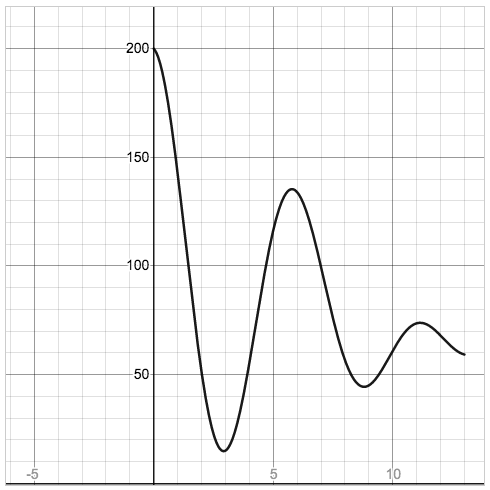
\includegraphics[scale=.3]{2_5_bungee}
	
\item Suppose the hight of a ball thrown into the air is given by $h(t)=-4.9t^2+12t+1.5$.
	\begin{enumerate}
	\item Use calculus to compute when the ball is traveling upward.
	\vfill
	\item Use calculus to compute when the trajectory of the ball is concave down.

	\end{enumerate}
	 
\end{enumerate}
\end{document} 

%%%%%%%%%
\item Suppose $f(t)$ is graphed below. Sketch a graph of $f''(t)$. If $f(t)$ represents the position of an object as a function of time, what does $f''(t)$ represent? \\
\includegraphics [height=80mm, width=120mm]{secondder}
		\vfill
\newpage
\item Sketch a graph of a function with each of the given properties, or explain why no such function exists.\\
\includegraphics [height=90mm, width=140mm]{secondderitvative}

\item A car is driving down Willamette Blvd. The graph and table describe its location ($s$ in feet) as a function of time ($t$ in seconds). \\	
\includegraphics [height=50mm, width=70mm]{car}

\begin{tabular}{l| cccc cccc cccc c}
 $s$& 0 & 1 & 2 & 3 &4 &5 &6 &7 &8 &9 &10 &11 &12  \\
 \hline
 $s(t)$& 10 & 15 & 21 & 31 &45 &70 &95 &110 &120 &125 &125 &130 &150  \\

\end{tabular}

\begin{enumerate}
	\item Give a general description of the motion of the car. What features are of particular interest?
	\vfill
	\item On what intervals is $s''(t)$ positive? When is $s''(t)$ zero? When is $s''(t)$ negative? Interpret the meaning of these intervals in the context of the problem.
	\vfill
	\item Sketch a graph of $s'(t)$. Sketch a graph of $s''(t)$.
	\end{enumerate}
	


\begin{tcolorbox}
\textbf{Warm-up: } Solve the following equations for $t$.
\begin{multicols}{2}
\begin{enumerate}
\item $(t+1)^2=9$
\item $tx+x^2=5$
\end{enumerate}
\end{multicols}
\end{tcolorbox}

MINIPAGE
\noindent\begin{minipage}{0.3\textwidth}% adapt widths of minipages to your needs
try 1
\end{minipage}%
\hspace{40mm}
\begin{minipage}{0.6\textwidth}
a) $f'(2)=$\\\

b) $f'(4)=$\\

c) $f'(6)=$\\

d) $f'(7)=$\\

e) $f'(8)=$
\end{minipage}
